\documentclass[12pt, letterpaper, twoside]{article}
\usepackage[T1]{fontenc}
\usepackage[utf8]{inputenc}
\usepackage[russian]{babel}
\usepackage[a1paper]{geometry}
\geometry{papersize={29.7 cm, 25.0 cm}}
\usepackage{graphicx}
\title{DIFFERENCIATOR MACHINE}
\author{Makson from 225}
\date{}
\begin{document}
\maketitle
\newpage
\section{Showing the source tree}
\begin{center}
Your function is $F = e^{2 \cdot x}$\newline 
\begin{figure}
\begin{center}
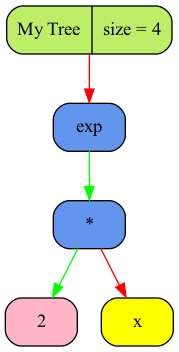
\includegraphics [scale = 0.4]{graphics/graph1.png}
\caption{Get your funtion}
\end{center}
\end{figure}
\end{center}
\newpage
\section{Finding function at the point}
\begin{center}
Your function is $F = e^{2 \cdot x}$.
The value of your function at 0: $ F(0) = 1 $
\end{center}
\newpage
\section{Getting derivative}
\begin{center}
$(e^{2 \cdot x})' = e^{2 \cdot x} \cdot (0 \cdot x + 2 \cdot 1)$\\
Oh shit, it so deep...\\
$(e^{2 \cdot x})' = e^{2 \cdot x} \cdot (0 + 2)$\\
Oh shit, it's depper than before\\
$(e^{2 \cdot x})' = e^{2 \cdot x} \cdot 2$\\
Fuck, i'm cumming from this calculations\\
$(e^{2 \cdot x})' = e^{2 \cdot x} \cdot 2$\\
It was the best sex.., xm, differenciation ever
\end{center}
\newpage
\section{Getting derivative at the point}
\begin{center}
Your function is $F = e^{2 \cdot x} \cdot 2$.
The value of your function at 0: $ F(0) = 2 $
\end{center}
\newpage
\section{Showing the Diff tree}
\begin{center}
Your function is $F = e^{2 \cdot x} \cdot 2$\newline 
\begin{figure}
\begin{center}
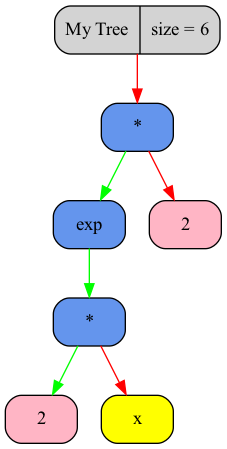
\includegraphics [scale = 0.4]{graphics/graph2.png}
\caption{Get your funtion}
\end{center}
\end{figure}
\end{center}
\newpage
\section{Makclurin formula}
I like big expressions XD\\
\begin{center}
$e^{2 \cdot x} =  1 +  2x + \frac{4x^{2}}{2!} + \frac{8x^{3}}{3!} + \frac{16x^{4}}{4!} + \frac{32x^{5}}{5!} + o(x^{5}) $
\end{center}
\end{document}